\documentclass[12pt,reqno, a4]{amsart}
\setlength{\topmargin}{0cm}\setlength{\textheight}{205mm}
\setlength{\oddsidemargin}{0.5cm} \setlength{\evensidemargin}{0.5cm}
\setlength{\textwidth}{155mm}
%%%%%%%%%%%%%%%%%%%%%%%%%%%%%%%%%%%%%%%%%%%%%%%%%%%%%%%%%%%%%%%%%%%%%%%%%%%%%%%%%%%%%%%%%%%%%%%%%%%%%%%%%%%%%%%%%%%%%%%%%%%%%%%%%%%%%%%%%%%%%%%%%%%%%%%%%%%%%%%%%%%%%%%%%%%%%%%%%%%%%%%%%%%%%%%%%%%%%%%%%%%%%%%%%%%%%%%%%%%%%%%%%%%%%%%%%%%%%%%%%%%%%%%%%%%%
\usepackage{amssymb}\usepackage{cancel}
%\usepackage{txfonts}
\usepackage{amsfonts}
\usepackage{mathrsfs}
\usepackage{amsmath}
\usepackage{graphicx}
\usepackage{hyperref}
\usepackage{float}
\usepackage{epstopdf}
\usepackage{color}
\usepackage{bm}
\usepackage{comment}
\usepackage{soul}
\usepackage{esint}
\usepackage{amsthm}
\usepackage{setspace}
\usepackage[backend=biber,style=numeric, sorting=none]{biblatex}
\usepackage{caption}

 \addbibresource{citation.bib}


\setstretch{1}

\newcommand\N{\ensuremath{\mathbb{N}}}
\newcommand\R{\ensuremath{\mathbb{R}}}
\newcommand\Z{\ensuremath{\mathbb{Z}}}
\renewcommand\O{\ensuremath{\emptyset}}
\newcommand\Q{\ensuremath{\mathbb{Q}}}
\newcommand\C{\ensuremath{\mathbb{C}}}
\newcommand{\E}[1]{\ensuremath{\mathbb{E}\left( #1 \right)}}
\newcommand\pr[1]{\ensuremath{\mathbb{P}\left (#1 \right)}}

\let\implies\Rightarrow
\let\impliedby\Leftarrow
\let\iff\Leftrightarrow
\let\e\varepsilon


%quick set notation from math tool\textbf{}
\allowdisplaybreaks
\newtheorem{theorem}{Theorem}[section]
\newtheorem{proposition}[theorem]{Proposition}
\newtheorem{lemma}[theorem]{Lemma}
\theoremstyle{definition}
\newtheorem{definition}[theorem]{Definition}
\newtheorem{corollary}[theorem]{Corollary}
\newtheorem*{remark}{Remark}
\newtheorem*{remarks}{Remarks}
\newtheorem*{example}{Example}

\newtheorem{conjecture}[theorem]{conjecture}
\newtheorem{problem}[theorem]{Problem}
\newtheorem{thm}{Theorem}

\numberwithin{equation}{section}
\newenvironment{acknowledgement}{\smallskip{\sc Acknowledgement.}\rm}{\smallskip}
\def\limfunc#1{\mathop{\mathrm{#1}}}
\usepackage{algorithm}
\usepackage{algpseudocode}
\renewcommand{\arraystretch}{1.25}
\usepackage{bbm}

\bibliography{citation}


\begin{document}
\title{The Friendship Paradoxes}
\author{Nguyen Viet Duc}

\maketitle
\begin{abstract}
    This paper discusses the Friendship Paradoxes - a set of classical results at the intersection of graph theory and network science. There are two main versions of the Friendship Paradox: the original one due to Feld \cite{feld_why_1991} states that the expected degree of a randomly chosen vertex is smaller than that of a randomly chosen neighbor (precisely, a random vertex chosen from a randomly chosen edge), while the other (supposedly) due to Hofstad \cite{hofstad_random_2016} shows that a randomly chosen vertex have fewer neighbors than its immediate neighbors on average. In common parlance, the Friendship Paradox asserts that you have fewer friends than (your) friends on average. The paper rigorously formulate and prove both versions of paradox. It concludes with a brief discussion on the theoretical, and practical implications of the Friendship Paradoxes.
\end{abstract}
\tableofcontents

\section{Introduction}
The Friendship Paradox is a class of well-known results in graph theory and an empirically verified social phenomenon. In graph-theoretical terminology, it roughly states that the expected degree of a vertex is always smaller or equal to that of (its) neighbors. In social network literature, the paradox is the observation that an individual has fewer friends than (his/her) friends on average. 

Some of the earliest scientific record of what is now known as Friendship Paradox is due to Feld and Grofman \autocite{feld_variation_1977}, where they pointed out that on average students found themselves in larger classes than the empirical mean class size. In a 1991 paper, Feld \cite{feld_why_1991} published the first mathematical treatment of the phenomenon where `the
 mean number of friends of friends is always greater than the mean number of friends of individual' with a simple argument capturing the  underlying the paradox: a sampling bias where individuals with more friends are over-represented in the \textit{`distribution of friends of friends'}, as compared to the \textit{`distribution of friends of individuals'}. In this study, Feld also empirically verified a stronger assertion - that most people have fewer friends than \textit{their} friends - but did not offered any mathematical explanation as to why this is the case. This stronger version of the friendship paradox is established allegedly\footnote{Hofstad claims in his book `Random Graph and Complex Network'\cite{hofstad_random_2016} that he came up with the result independently, but was not sure if he was the first to do it.} by Hofstad \cite{hofstad_random_2016}, which shows that the expected degree of a vertex is always smaller or equal to its \textit{own} immediate neighbor. These theoretical results have inspired a slew of empirical experiments in the past 2 decades, which in turn lend evidence to the existence of the Friendship Paradox in real life. Most notably, a 2011 analysis \cite{ugander_anatomy_2011} of 721 millions Facebook users (roughly $10\%$ of the population at the time) found that the average number of friends of an user is 190, while his/her friends average 635.

 In what follows, a mathematical formulation of a social network - the domain which the Friendship Paradox originates from and is often studied in - will be constructed in Section 2. We then formally state and prove the two aforementioned versions of the Friendship Paradox in Section 3 and Section 4. A brief discussion on the theoretical and practical implications of the Friendship Paradox in Section 5 conclude the paper.
\section{Mathematical Formulation}
    We begin by defining the mathematical tools which we would use to describe the Friendship Paradox.
\begin{definition}[Finite Simple Graph]
    A finite graph $G$ is a pair $(V, E)$ where
    \begin{itemize}
        \item $V = \{v_1,v_2, \dots, v_n\}$ is a finite collection of vertices;
        \item $E = \left \{\{v_i,v_j \right \} \mid (i \neq j) \land  (v_i, v_j \in V)\}$ is a collection of unordered pairs of distinct vertices in $V$.
    \end{itemize}
\end{definition}
\begin{remark}
    A rigorous definition of a graph considers $E$ as a collection of \textit{edges} - mathematical abstractions representing a `relation' between \textit{vertices} (which are themselves another mathematical abstraction), and involves an \textit{incidence function} $\phi: E \to V \times V$ that associates an edge $e_i \in E$ with pairs of vertices in $V$. Such a treatment, however, is unnecessarily complicated for our purpose. 
\end{remark}
In essence, a graph is a mathematical construction that describe collections of objects which are in some way related to each other. The general definition of \textit{finite simple graph} provided above gives it great descriptive power to model numerous empirical networks. For example, the set of vertices $V$ can include train stations, cells, or countries while the set of edges $E$ can be railways, cell-cell interactions, or diplomatic ties. Our model of the Friendship Paradox consider a vertex $v_i$ as individuals, while an edge $\{v_i, v_j\}$ as the mutual friendship between $v_i$ and $v_j$. The following definition describe the friends and the number of friends of an individual in a social network. 
\begin{definition}[Neighborhood]
    The \textit{neighborhood} of a vertex $v_i \in V$ is the set 
    \[
    \mathcal{N}(v_i) = \left \{v_j \mid \{v_i, v_j \} \in E\right  \}.
    \]
    An element in $\mathcal{N}(v_i)$ is called a \textit{neighbor} of $v_i$.
\end{definition}
\begin{definition}[Vertex Degree]
    The \textit{degree} $d(v_i)$ of a vertex $v_i \in V$ is the number of neighbors of $v_i$, that is,
    \[d(v_i) =  \left | \mathcal{N}(v_i) \right | \]
\end{definition}


\begin{example}
    Consider a social situation described by the following \textit{adjacency matrix}
    
    \begin{table}[h]
        \centering
        \begin{tabular}{|c|c|c|c|c|}
        \hline
             & \textbf{A} & \textbf{B} & \textbf{C} & \textbf{D} \\ \hline
           \textbf{A}  & 0 & 1 & 1 & 1 \\ \hline
           \textbf{B} & 1 & 0 & 0 & 1\\ \hline
           \textbf{C} & 1 & 0 & 0 & 0\\ \hline
           \textbf{D} & 1 & 1 & 0 & 0 \\ \hline
        \end{tabular}
    \end{table}
     \noindent where $a_{AB} = 1$ (element on row $A$, column $B$) means there is an edge between $A$ and $B$(or that $A$ and $B$ are friends). Such a situation can be graphically represented by the figure below
     \begin{center}
         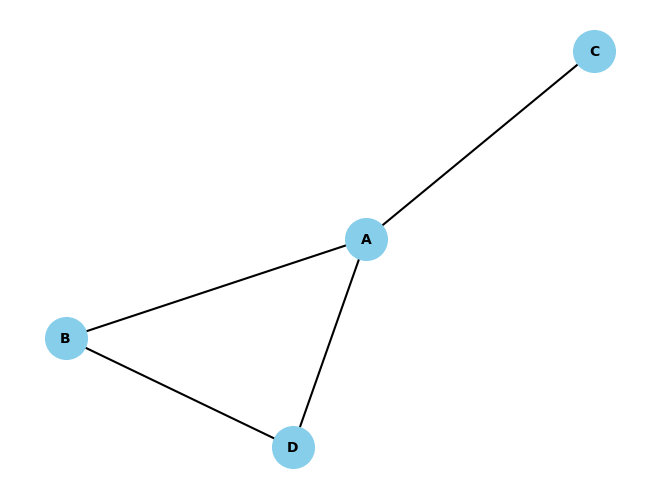
\includegraphics[width = 0.6\textwidth]{illustration/example graph.png}
     \end{center}
     The neighborhood (set of friends) of B is \(\mathcal{N}(B) = \{A ; D\}\) and the degree (number of friends) of $C$ is $d(C) = |\mathcal{N}(C)| = |\{A\}| = 1$.
\end{example}
\section{The Weak Friendship Paradox}
The original rendition of the Friendship Paradox due to Feld \cite{feld_why_1991} states that `the average number of friends of an individual is smaller or equal to that of friends'. In other words, the expected number of friends of an individual \textit{engaged in a random friendship} (referred to as `friends' by Feld) is higher than that of a random individual\footnote{Hereafter I refer to this phenomenon as the \textit{Weak Friendship Paradox}}. The following theorem describes this observation precisely using the graph-theoretical tools we just laid out.
\begin{theorem}[The Weak Friendship Paradox] \label{thm:1}
    Let $G = (V, E)$ be a finite simple graph. Uniformly choose an edge at random, then choose a vertex uniformly at random from the two vertices that the chosen edge connects. Denote the degree of the chosen vertex $D_n^*$, then 
    \begin{equation}
        \E{D_n^*} \geq \E{D_n}
    \end{equation}
    where $D_n$ is the degree of a vertex chosen uniformly at random.
\end{theorem}
\begin{remark}
    Note that $D_n^*$ and $D_n$ are both random variables that maps the randomly chosen vertex (of the same graph but from two different random process) to its corresponding degree. The randomly chosen edge corresponds to a \textit{random friendship}, while $\E{D_n^*}$ represents the expected number of friends of an individual engaged in a random friendship, and $\E{D_n}$ represents the expected number of friends a random individual. 
\end{remark}
The Weak Friendship Paradox can be derived in a straightforward manners using arithmetic techniques similar to ones used by Feld \autocite{feld_why_1991} or Cantwell \cite{cantwell_friendship_2021}. Here, I will take a short detour to describe the probability mass distribution of $D_n^*$. An understanding of the distribution of $D_n^*$ not only immediately leads to a proof of $(3.1)$, but also rewards us with tractable intuition which may otherwise be inaccessible.
\begin{lemma} \label{thm: lemma 1}
     The probability mass function of $D_n^*$ is 
    \begin{equation}
        \pr{D_n^* = k} = \frac{k}{\E{D_n}} \pr{D_n = k} 
    \end{equation}
\end{lemma}
\begin{proof}[Proof of Lemma \ref{thm: lemma 1}]
    Let $K = \{k_1, k_2, \dots, k_m\} \subseteq V$ be the set of vertices with degree $k$. Denote the $v^*$ to be the vertex chosen by first choosing an edge at random, then randomly choosing one of its vertices. We see that 
    \[
    \pr{D_n^* = k} = \pr{v^* \in K} = \pr{\bigcup_{1}^m v^* = k_i} 
    \]
    where $v^* = k_i$ denotes the event that the $k_i$ vertex is chosen. Since the events $v^* = k_i \ (i = 1, 2, \dots, m)$ are disjoint,
    \[
    \pr{D_n^* = k} = \sum_{1}^m \pr{v^* = k_i}
    \]
    Observe that for arbitrary $k_i \in K$ 
    \[
    \pr{v^* = k_i} = \frac{k}{|E|} \times \frac{1}{2}
    \]
    where $k/|E|$ denotes the probability that one of $k$ edges connected to $k_i$ are chosen in the first step, and $1/2$ is the probability that $k_i$ is chosen out of the two vertices incident to the chosen edge. We thus have
    \[
    \pr{D_n^* = k} = \frac{mk}{2|E|} = \frac{k}{2|E|/n} \times \frac{m}{n}.
    \]
    Recognize that \begin{align*}
        \E{D_n} &= \frac{1}{n} \times \sum_{v \in V} d(v) = \frac{2|E|}{n};\\
        \pr{D_n = k} &= \frac{|K|}{|V|} = \frac{m}{n},
    \end{align*}
    where the first identity comes from the fact that \textit{the sum of the degrees of vertices in a graph is 2 times its total number of edges}, and the second is the probability that a randomly chosen vertex is one of $m$ vertices with degree $k$.\\
    We thus obtain
    \[
    \pr{D_n^* = k} = \frac{k}{\E{D_n}} + \pr{D_n = k}.
    \]
\end{proof}
    We see from $(3.2)$ that while the edge is randomly chosen, the vertex $v^*$ is not chosen uniformly at random from the collection of vertices. Rather, the higher the degree $k$ of a vertex, the higher the probability that it would be chosen. This is an example of a `sampling bias', where the random process that first chooses an edge is biased toward vertices with more edges attached to it (higher degree). And with this, we also have all the tools we need to prove the Weak Friendship Paradox.
\begin{proof}[Proof of Theorem \ref{thm:1}]
    By definition we have \[
\E{D_n^*} = \sum_k k \times \pr{D_n^* = k} = \frac{1}{\E{D_n}} \sum_k k^2 \pr{D_n = k} = \frac{\E{D_n^2}}{\E{D_n}}.
\]
Because $\E{D_n^2} = \E{D_n}^2 + \text{Var}(D_n)$, we have
\[
\E{D_n^*} = \E{D_n} + \frac{\text{Var}(D_n)}{\E{D_n}} \geq \E{D_n}
\]
where the inequality follows from the fact that $\text{Var}(D_n) \geq 0$.
\end{proof}
\section{The Strong Friendship Paradox}
A (somewhat) stronger version of Feld's original Friendship Paradox\footnote{Hereafter I call this the \textit{Strong Friendship Paradox}.} due to Hofstad \cite{hofstad_random_2016} states that the expected number of friends of a randomly chosen individual is smaller or equal to that of his/her randomly chosen friend. The distinction between this and Feld's Weak Friendship Paradox is that the latter compares the expected number of friends of an individual with that of a general `friends' in the network, while the former compares directly with that of his/her immediate inner circle.
\begin{theorem}[The Strong Friendship Paradox] \label{thm:2}
    Let $G = (V, E)$ be a finite graph. Assume that $d(v) \geq 0$ for all $v \in V$. Draw a vertex $u$ uniformly at random from $V$, and then choose a vertex $v$ also uniformly at random from the neighborhood $\mathcal{N}(u)$. Let $X_1$ and $X_2$ be the degree of $u$ and $v$ respectively. Then
    \begin{equation}
        \E{X_2} \geq \E{X_1}
    \end{equation}
\end{theorem}
\begin{remark}
    In this setting, $u$ is a randomly chosen individual, $v$ is his/her randomly chosen friends. The Strong Friendship Paradox states that the expected number of friends of $v$ is at least as small as that of $u$.
\end{remark}
Similar to the Weak Friendship Paradox, the proof for Theorem \ref{thm:2} follows trivially once we have obtained the probability mass distribution of $X_2$ and $X_1$. However, since the choice of $v$ and, by extension, $X_2$ is dependent upon the choice of $u$ as well as the structure of the graph itself (for example, is there a vertex $v$ with degree $X_2$ that is connected to the vertex $u$ with degree $X_1$? If yes, how many?), we must derive a joint distribution of $X_1$ and $X_2$.
\begin{lemma} \label{lemma 2}
    The joint distribution of $X_1$ and $X_2$ is 
    \begin{equation}
        \pr{X_1 = k, X_2 = l} = \frac{1}{n} \sum_{(u, v) \in E'} \mathbbm{1}_{d(u) = k, d(v) = l} \frac{1}{d(u)}
    \end{equation}
    where $E'$ is the set of \textit{directed edges} generated from $E$, that is, $E'$ is an set of ordered pairs of vertices \[
    E' = \{(v_i, v_j), (v_j, v_i) \mid \{v_i, v_j\} \in E\},
    \] and $\mathbbm{1}_{d(u) = k, d(v) = l}$ is the indicator random variable associated with the event \[d(u) = k, d(v) = l.\]
\end{lemma}
\begin{proof}[Proof of Lemma \ref{lemma 2}]
    Fix $k$ and $l$. Let $A = \{(a,b) \mid (a,b) \in E' \land d(a) = k \land d(b) = l\}$. In words, $A$ is the set of directed edges in $E$ where the first endpoint has degree $k$ and the second endpoint has degree $l$.
    There are  
    \[
    \sum_{(u, v) \in E'} \mathbbm{1}_{d(u) = k, d(v) = l} 
    \] elements in $A$. Consider an arbitrary $(a^*, b^*) \in A$.  The probability that the first chosen vertex is $a^*$ is
    \[\pr{u = a^*} = \frac{1}{n},
    \] since $u$ is chosen uniformly at random from a set of $n$ vertices. The probability that the second chosen vertex is $b^*$ (denoted $v = b^*$) is \[\frac{1}{k} = \frac{1}{d(a^*)} = \frac{1}{d(u)}\] since $v$ is chosen uniformly at random from the $d(u)$ neighbors of $u$. We thus have
    \[
    \pr{u = a^*, v = b^*} = \frac{1}{n} \times \frac{1}{d(u)}
    \]
    Recognize that
    \[
    \pr{X_1 = k, X_2 = l} = \pr{(u,v) \in A} = \pr{\bigcup_{(a,b) \in A} (u = a, v = b)}.
    \]
    Since for for each pair $(a,b) \in A$, the event $u = a, v = b$ (in words, the event that the first chosen vertex is $a$, and the second chosen vertex is $b$) is disjoint, and also equally likely (as is shown above), we have
    \begin{align*}
            \pr{X_1 = k, X_2 = l} &= \sum_{(u, v) \in E'} \mathbbm{1}_{d(u) = k, d(v) = l} \pr{u = a^*, v = b^*}\\ &= \sum_{(u, v) \in E'} \mathbbm{1}_{d(u) = k, d(v) = l}  \frac{1}{n} \times \frac{1}{d(u)} \\& = \frac{1}{n} \sum_{(u, v) \in E'} \mathbbm{1}_{d(u) = k, d(v) = l} \frac{1}{d(u)}
    \end{align*}
    % Fix $k$ and $l$. Consider the random process where we randomly choose a directed vertex $(u, v)$ from the directed edge set $E'$. The event $(X_1 = k, X_2 = l)$ is the event\footnote{Since $u$ and $v$ are both chosen uniformly at randomly given their respective sample space - $V$ and $\mathcal{N}(u)$.} where a randomly chosen directed edge from $E'$ has its first endpoint with $k$ degrees, and its second endpoint with $l$ degrees.
    % First acknowledge that 
    % \[
    % \pr{X_1 = k,X_2 = l} = \pr{X_2 = l \mid X_1 = k}
    % \]
    % since $X_2$ always evaluated once $X_1$ is determined.\\
    % The random process described in Theorem \ref{thm:2} is thus analogous to uniformly draw a directed\footnote{Because the order of the degree of $u$ and $v$ matters, we need to consider direction.} edge $(u,v)$ from $E'$ where $d(u) = k$. In total, there are 
    % \[
    % n \times d(u),
    % \]
    % corresponding to $n$ number of ways we can choose $u$, and $d(u)$ numbers of way we can choose $v$ given $u$ already chosen.
    % The number of valid ways, however , is the number of $(u, v)$ where $d(u) = k$, $d(v) = l$, and $v \in \mathcal{N}(u)$, which is described by the identity
    % \[
    % \sum_{(u, v) \in E'}  \mathbbm{1}_{d(u) = k, d(v) = l}.
    % \]
    % Now, since each of the directed edges are equally likely, we thus have
    % \begin{align*}
    %     \pr{X_2 = l \mid X_1 = k} &= \frac{\sum_{(u, v) \in E'}  \mathbbm{1}_{d(u) = k, d(v) = l}}{n \times d(u)} \\ &= \frac{1}{n} \sum_{(u, v) \in E'}  \mathbbm{1}_{d(u) = k, d(v) = l} \frac{1}{d(u)}.
    % \end{align*}
    % Since \(\pr{X_1 = k,X_2 = l} = \pr{X_2 = l \mid X_1 = k}\), we obtain Lemma \ref{lemma 2}.
\end{proof}
From Lemma 2, we can derive the probability distribution, and expectation of $X_1$, which can then be used to calculate their respective expectations.
\begin{proof}[Proof of Theorem \ref{thm:2}]
    From Lemma \ref{lemma 2}, the probability distribution of $X_1$ and $X_2$ is 
    \begin{align*}
        \pr{X_1 = k} &= \sum_{l} \pr{X_1 = k, X_2=l} \\&= \sum_{l} \frac{1}{n} \sum_{(u, v) \in E'}\mathbbm{l}_{d(u) = k, d(v) = l} \frac{1}{d(u)} \\&= \frac{1}{n} \sum_{(u, v) \in E'}\sum_{l} \mathbbm{l}_{d(u) = k, d(v) = l} \frac{1}{d(u)}\\
        \pr{X_2 = l} &= \sum_{k} \pr{X_1 = k, X_2=l} \\ & = \sum_k \frac{1}{n} \sum_{(u, v) \in E'} \mathbbm{l}_{d(u) = k, d(v) = l} \frac{1}{d(u)} \\&= \frac{1}{n} \sum_{(u, v) \in E'} \sum_{k} \mathbbm{l}_{d(u) = k, d(v) = l} \frac{1}{d(u)}
    \end{align*}
    where the change in the order of the sums is possible because, intuitively
    \[
    \sum_l \sum_{(u, v) \in E'} \mathbbm{1}_{d(u) = k, d(v) = l}\ ,\  \sum_{(u, v) \in E'}\sum_{l} \mathbbm{l}_{d(u) = k, d(v) = l}
    \] denote the number of directed edges $(u,v)$ while
    \begin{align*}
            \sum_k \sum_{(u, v) \in E'} \mathbbm{1}_{d(u) = k, d(v) = l} \frac{1}{d(u)} \ ; \ \sum_{(u, v) \in E'} \sum_k   \mathbbm{1}_{d(u) = k, d(v) = l} \frac{1}{d(u)} 
    \end{align*}
    both denotes the number of directed edges $(u, v)$ with $d(v) = l$. Technically speaking, the change of the order of sum is possible because \textit{at each component of the sum on the right hand sides, the value $d(u) = k$ is fixed for some k}.\\
    Recognize that for any \textit{chosen}\footnote{We now consider $u$ and $v$ to be some fixed vertices, we deal first with the randomness of their degrees} $u$ and $v$, \[\sum_{k, l} \mathbbm{1}_{d(u) = k, d(v) = l} = 1 \times \sum_{k,l} \pr{d(u) = k, d(v) = l} =  1. \] We can thus derive the expectation of $X_1$ where
\begin{align*}
    \E{X_1} &= \sum_{k} k \times \frac{1}{n} \sum_{(u, v) \in E'} \sum_{l}\mathbbm{l}_{d(u) = k, d(v) = l} \frac{1}{d(u)}\\
    & = \frac{1}{n}\sum_{(u, v) \in E'} \sum_k \sum_l k \times\mathbbm{l}_{d(u) = k, d(v) = l} \frac{1}{d(u)} \\
    & = \frac{1}{n} \sum_{(u, v) \in E'} \sum_{k, l} \mathbbm{l}_{d(u) = k, d(v) = l} \frac{k}{d(u)} \\
    &= \frac{1}{n} \sum_{(u, v) \in E'} \sum_{k,l} \mathbbm{1}_{d(u) = k, d(v) = l}.\\
    & =  \frac{1}{n} \sum_{(u, v) \in E'} 1
\end{align*}
because at each component of the sum on the RHS, the value $d(u) = k$ is fixed. Similarly, the expectation of $X_2$ is
\begin{align*}
    \E{X_2} & = \sum_l l \times \frac{1}{n} \sum_{(u, v)  \in E'} \sum_{k}\mathbbm{l}_{d(u) = k, d(v) = l} \frac{1}{d(u)}\\
    & =  \frac{1}{n}\sum_{(u, v) \in E'} \sum_l \sum_{k} l \times \mathbbm{l}_{d(u) = k, d(v) = l} \frac{1}{d(u)}\\
    & = \frac{1}{n}\sum_{(u, v) \in E'} \sum_{k, l}\mathbbm{l}_{d(u) = k, d(v) = l} \frac{l}{d(u)}\\ & = \frac{1}{n} \sum_{(u, v) \in E'} \sum_{k,l} \mathbbm{l}_{d(u) = k, d(v) = l} \frac{d(v)}{d(u)} \\ & = \frac{1}{n} \sum_{(u, v) \in E'} \frac{d(v)}{d(u)} \sum_{k,l} \mathbbm{l}_{d(u) = k, d(v) = l}\\
    & = \frac{1}{n} \sum_{(u,v) \in E'} \frac{d(v)}{d(u)}
\end{align*} where, again, we have change $d(v)/d(u)$ to the front because within the $\sum_{(u,v) \in E'}$ sum, the $u$ and $v$ is fixed ($k$ and $l$ changed).
From the Cauchy-Schwarz Inequality, we have \[
1 \leq \frac{1}{2} \left (\frac{d(v)}{d(u)} + \frac{d(u)}{d(v)} \right )
\] for any vertices $u, v$. This implies
\[
\E{X_1} \leq \frac{1}{n} \sum_{(u, v) \in E'}\frac{1}{2}\left (\frac{d(v)}{d(u)} + \frac{d(u)}{d(v)} \right ) = \frac{1}{n} \sum_{(u, v) \in E'} \frac{d(v)}{d(u)} = \E{X_2},
\]
where the penultimate equality follows from the fact that \[
\sum_{(u, v) \in E'} \frac{d(v)}{d(u)} = \sum_{(u, v) \in E'}\frac{d(u)}{d(v)}.
\]
\end{proof}
\section{Empirical Experiment}
I verify this phenomenon in empirical network data, sourced from Rozemberczki et al. \cite{rozemberczki_characteristic_2020}. My network (image below) contains 7,624 nodes (representing LastFM users in Asia) and 27,806 undirected edges (mutual follower relationships). I randomly sample a node from the data 5000 times and record their degrees. I then  randomly sample a node from a randomly chosen edge (Feld's Friendship Paradox), and randomly sample a neighbor of a randomly chosen node (Hofstad's Friendship Paradox). The following figure illustrates that the mean (expected value) of the number of friends of a selected individual is smaller than that of a randomly selected friend (Felds), or his/her own friends (Hofstad's).

\begin{figure}[H]
  \centering  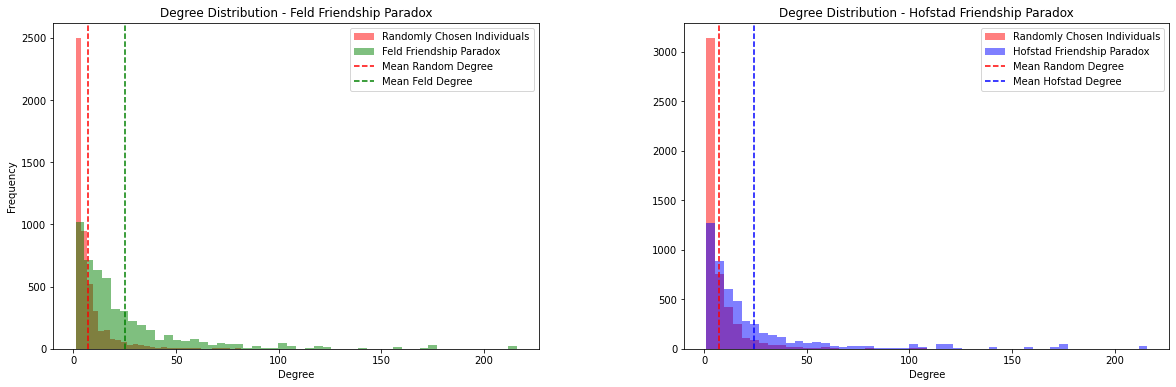
\includegraphics[width=\textwidth]{illustration/experiment_result.png}
  \caption{Experiment Result}
\end{figure}


\section{Discussion}
From a purely theoretical point of view, the presented two versions of the Friendship Paradox not only delivers tractable intuition regarding the `sampling' bias, but also hints at a deeper mathematical world where these phenomenon can be dissected and analyzed. The random variable $D_n^*$ is defined in our formulation of the \textit{Weak Friendship Paradox} is an example of a \textit{size-biased random variable}, which is rigorously defined as a random variable $X^*$ corresponding to a non-negative random variable $X$ where \[
\pr{X^* \leq x} = \frac{\E{X\mathbbm{1}_{X \geq x}}}{\E{X}}.
\]
\begin{figure}
  \centering  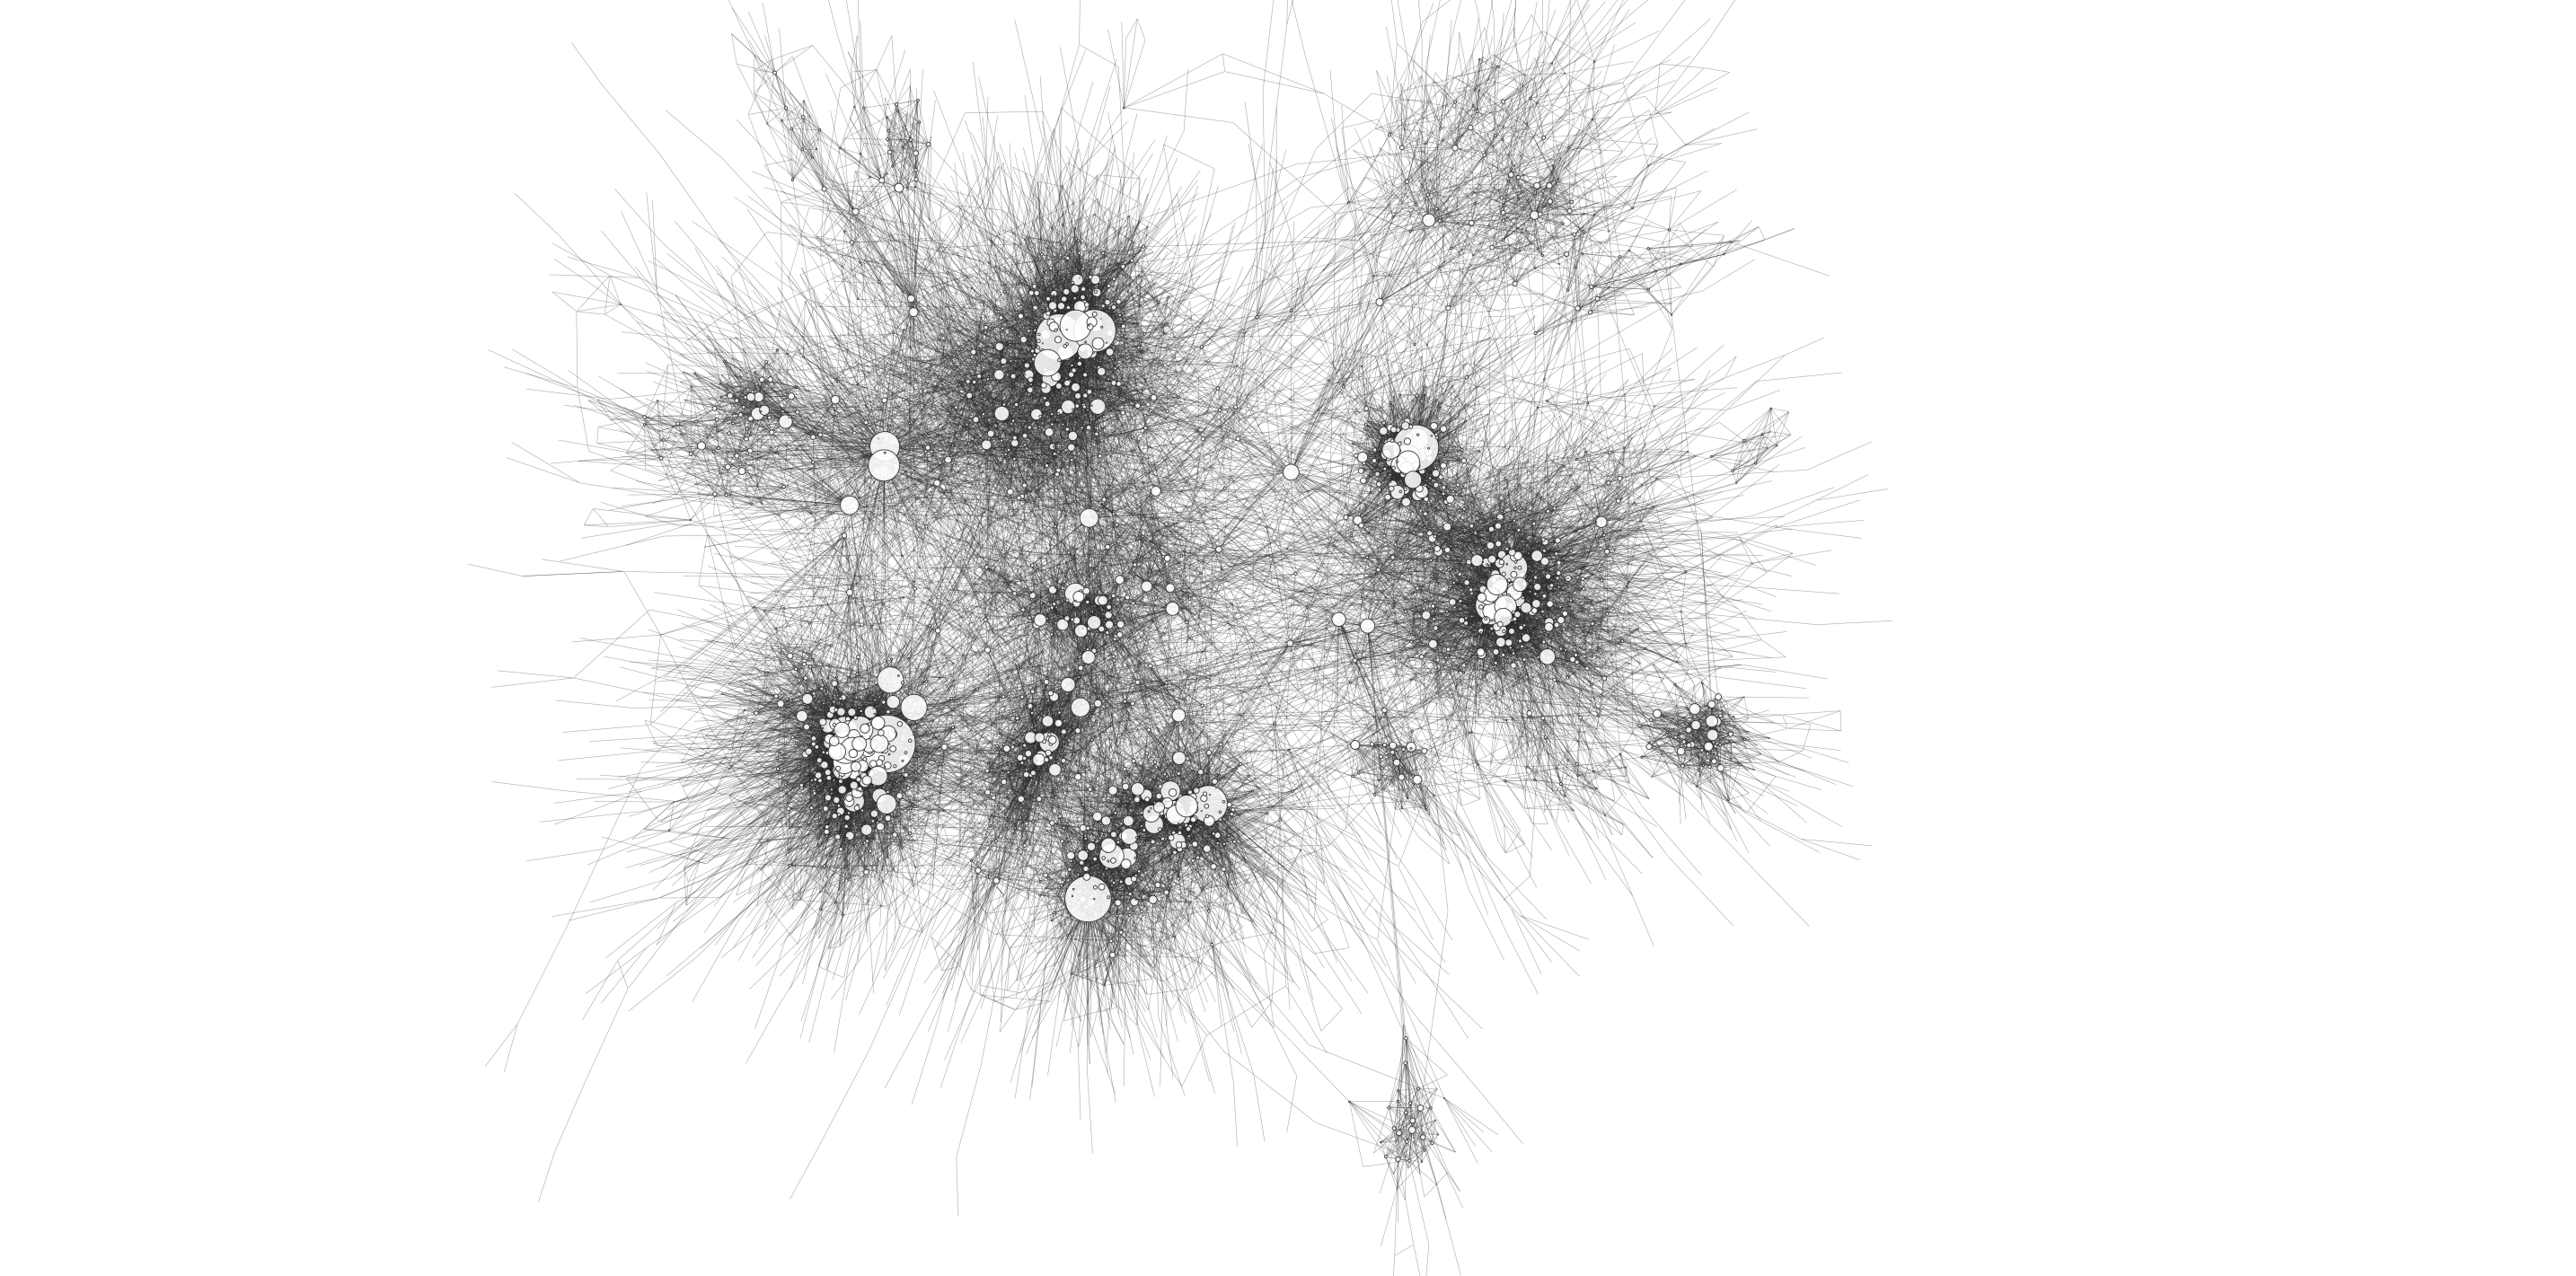
\includegraphics[width = 1.2\textwidth]{illustration/lastfm_network.png}
  \caption{LastFM Network (illustrated with Cytoscape)}
\end{figure}
In the \textit{Weak Friendship Paradox}, $D_n^*$ is the \textit{size-biased} version of $D_n$. Size-biased random variables provides us meaningful tools to describe sampling biases in experimental design, while at the same time teasing at an even more profound mathematical concept of \textit{stochastic ordering}.
\begin{definition}[Stochastic Ordering]
    Let $X$ and $Y$ be two random variables. The random variable $X$ is stochastically smaller than the random variable $Y$ when, for every $x \in \R$, the inequality
    \[
    \pr{X \geq x} \geq \pr{Y \leq x}
    \] holds. We write $Y \succeq X$
\end{definition}
\noindent In our case, the random variable $D_n$ is stochastically smaller than $D_n^*$, that is, $D_n^* \succeq D_n$. In essence, \textit{stochastic ordering} are binary relations defined on a probability distribution. This concept extends the intuitive notions of order from the real line to probability distributions, thus allowing us to make more nuanced comparison regarding a probability distribution, as opposed to having to rely on the often-times biased test statistics such as the mean or the median. Already, works applying \textit{stochastic ordering} to decison theory, financial optimization, and control theory are already under way.

Besides its connections to the aforementioned theoretical development in Probability Theory, the Friendship Paradox itself is also being extended and studied in more and more theoretically complicated models of social networks. A 2014 study by Eom and Jo \cite{eom_generalized_2014} described and empirically verified the \textit{Generalized Friendship Paradox}, which considered different network characteristics other than vertices' degrees. Observing cooauthorship networks of Physical Review journals and Google Scholar profiles, they found that phenomena in the form of a Friendship Paradox are found not only for the number of friends, but also the number of coauthor, the number of citations, and the number of publications of an individual. On the other hand, there have also been studies into directed models of the Friendship Paradox, where relationships are assumed not to be reciprocal, such as in the case of influencer - follower on social media. For example, Hodas et al. \cite{hodas_friendship_2013} found that, on average, those who you follow, and your followers on Twitter both have more friends, followers, and received more viral content than you. Another natural theoretical extension is to consider weighted forms of friendship paradox, where relationships (edges) are not homogeneous and are ascribed numerical values to describe their difference. A recent study by Ghasemian and Christakis \cite{ghasemian_enmity_2023} studied over 24,000 people in rural Hondoras and showed that the Friendship Paradox exists in mixed-world network, that is, social networks with both positive and negative (antagonistic) relationships. To use one of the results from this study as an example, this means that an individual's friends also typically has more enemies than he/she does.

The Friendship Paradoxes has found a wealth of applications across many domains. In their essence, the Friendship Paradox is a local property of an arbitrary network, and thus have sweeping generalization power for all things that are network-based. This descriptive power of the Friendship Paradoxes leads to one to predict, and ultimately manipulate the behavior of a network. For example, Christakis and Fowler monitored the flu status of a group of Harvard undergraduates and a subset of friends they named during the H1N1 pandemic in 2009 \cite{christakis_social_2010}. They found the group of friends got sick two weeks earlier than average. This result hints at a potential mechanism of an early warning system for contagious diseases. In social network, the Friendship Paradox also manifests in terms of the `majority illusion' \cite{lerman_majority_2016} and systematic bias \cite{jackson_friendship_2019} when people perceive certain social states, or personality traits such as extraversion, a higher rate tolerance to be more prevalent. Knowledge of the Friendship Paradox thus informs policymakers of potential ways to tackle these phenomena in an age where echo chambers and filter bubbles are rampant on social media, or can lend itself to be leveraged as potent marketing tools \cite{ben_sliman_asymmetric_2018} in the digital age.

\printbibliography
\end{document}